%%%%cls文件默认改用ctexart类,如果使用使用cctart类,请使用xelatex并修改SCIS2022cn.cls文件对应内容;
% !TEX encoding = UTF-8
% !TEX program = xelatex
%-----------------------------------------------------------------------
% 中国科学: 信息科学 中文模板, 请用 TexLive 编译
% http://scis.scichina.com
%-----------------------------------------------------------------------

\documentclass{SCIS2022cn}
%%%%%%%%%%%%%%%%%%%%%%%%%%%%%%%%%%%%%%%%%%%%%%%%%%%%%%%
%%% 作者附加的定义
%%% 常用环境已经加载好, 不需要重复加载
%%%%%%%%%%%%%%%%%%%%%%%%%%%%%%%%%%%%%%%%%%%%%%%%%%%%%%%

\usepackage[dvipsnames]{xcolor}  % 更全的色系
\usepackage{listings}  % 排代码用的宏包

%%%%%%%%%%%%%%%%%%%%%%%%%%%%%%%%%%%%%%%%
%% listings设置
%%%%%%%%%%%%%%%%%%%%%%%%%%%%%%%%%%%%%%%%
\lstset{
    language = Python,
    backgroundcolor = \color{yellow!10},    % 背景色:淡黄
    basicstyle = \small\ttfamily,           % 基本样式 + 小号字体
    rulesepcolor= \color{gray},             % 代码块边框颜色
    breaklines = true,                  % 代码过长则换行
    numbers = left,                     % 行号在左侧显示
    numberstyle = \small,               % 行号字体
    keywordstyle = \color{blue},            % 关键字颜色
    commentstyle =\color{green!100},        % 注释颜色
    stringstyle = \color{red!100},          % 字符串颜色
    frame = shadowbox,                  % 用(带影子效果)方框框住代码块
    showspaces = false,                 % 不显示空格
    columns = fixed,                    % 字间距固定
    %escapeinside={<@}{@>}              % 特殊自定分隔符:<@可以自己加颜色@>
    % morekeywords = {as},                % 自加新的关键字(必须前后都是空格)
    deletendkeywords = {compile}        % 删除内定关键字;删除错误标记的关键字用deletekeywords删!
}

%%%%%%%%%%%%%%%%%%%%%%%%%%%%%%%%%%%%%%%%%%%%%%%%%%%%%%%
%%% 开始
%%%%%%%%%%%%%%%%%%%%%%%%%%%%%%%%%%%%%%%%%%%%%%%%%%%%%%%
\begin{document}

%%%%%%%%%%%%%%%%%%%%%%%%%%%%%%%%%%%%%%%%%%%%%%%%%%%%%%%
%%% 作者不需要修改此处信息
\ArticleType{综述}
%\SpecialTopic{}
%\Luntan{中国科学院学部\quad 科学与技术前沿论坛}
% \Year{2022}
% \Vol{52}
% \No{1}
\BeginPage{1}
% \DOI{}
% \ReceiveDate{2021-xx-xx}
% \ReviseDate{2021-xx-xx}
% \AcceptDate{2021-xx-xx}
% \OnlineDate{2022-xx-xx}
% \AuthorMark{第一作者等}
% \AuthorCitation{作者1, 作者2, 作者3, 等}
% \enAuthorCitation{Xing M, Xing M M, Xing M, et al}
%%%%%%%%%%%%%%%%%%%%%%%%%%%%%%%%%%%%%%%%%%%%%%%%%%%%%%%

\title{Steiner Tree 问题综述}{Steiner Tree问题综述}

\entitle{Title}{Title for citation}

\author[1]{胡玉斌}{Yubin Hu1}{yubin.hu@bupt.edu.cn}

%若英文部分的emaillist太长需要换行的话,形式单独写在这里
%\enauthoremaillist{xingming1@xxxx.xxx, xingming2@xxxx.xxx, xingming3@xxxx.xxx, xingming4\\@xxxx.xxx, xingming5@xxxx.xxx}

%\comment{\dag~同等贡献}
%\encomment{\dag~Equal contribution}

\address[1]{北京邮电大学, 网络空间安全, 北京 100876}{北京邮电大学, Beijing {\rm 100876}, Country}

% \Foundation{国家自然科学基金 (批准号: 0000000, 0000000, 00000000)}

\abstract{本文主要介绍了斯坦纳树的问题背景,斯坦纳树的构造。并且在针对最小斯坦纳树的问题上,对多个Online Judge上的问题进行实验,分析思路并解决相关问题。结果表明,斯坦纳树问题在现实生活中应用的重要性以及未来学习的方向。}

% \enabstract{An abstract (about 200 words) is a summary of the content of the manuscript. It should briefly describe the research purpose, method, result and conclusion. The extremely professional terms, special signals, figures, tables, chemical structural formula, and equations should be avoided here, and citation of references is not allowed.}

\keywords{斯坦纳树,最小生成树,组合优化}

% \enkeywords{keyword1, keyword2, keyword3, keyword4, keyword5}

\maketitle

\section{引言}

%包括撰写文献综述的原因、意义、文献的范围、正文的标题及基本内容提要;
斯坦纳树(Steiner Tree Problem)问题,是组合优化中一个历史悠久的问题。
组合优化中研究的众多问题中就有斯坦纳树问题(STP)。自1970年成立以来,《网络》杂志上发表的许多文章激发了关于施泰纳树的新理论和计算研究:从近似算法、启发式、元启发式学,一直到基于(混合)整数线性规划、固定参数可及性或组合分支和绑定的精确算法。最近于2014年举行的第11次DIMACS实施挑战和2018年PACE挑战加强了施泰纳树的普遍适用性和相关性。\cite{1}
而如今,斯坦纳树问题在大规模集成电路设计、道路交通规划设计、无线传感器网络(物联网)等领域都有着广泛的运用。
此次综述将从斯坦纳树的问题背景,斯坦纳树的构造,算法实现以及现实问题的实际应用进行阐述。

%是文献综述的主要内容,包括某一课题研究的历史+(寻求研究问题的发展历程)、现状、基本内容+(寻求认识的进步),+研究方法的分析(寻求研究方法的借鉴),
%已解决的问题和尚存的问题,重点、详尽地阐述对当前的影响及发展趋势,这样不但可以使研究者确定研究方向,而且便于他人了解该课题研究的起点和切入点,
%是在他人研究的基础上有所创新;

\section{问题背景}

早在17世纪初,法国数学家费马就曾提出过费马点问题。
之后在19世纪初叶,著名学者斯坦纳,从这个非常简单却很有启示性的问题入手研究:
将三个村庄用总长为极小的道路连接起来。从数学上说,就是在平面内给定三个点 $A$、$B$、$C$ 找出平面内第四个点 $P$,使得和数 $a+b+c$ 为最短,这里 $a$、$b$、$c$ 分别表示从 $P$ 到 $A$、$B$、$C$ 的距离\cite{5}。

问题的答案是:如果三角形 $ABC$ 的每个内角都小于 $120^{\circ}$,那么 $P$ 就是使边 $AB$、$BC$、$AC$ 对该点所张的角都是 $120^{\circ}$ 的点。如果三角形 $ABC$ 的有一个角,例如 $C$ 角,大于或等于 $120^{\circ}$,那么点 $P$ 与顶点 $C$ 重合\cite{5}。

问题自然而然就可以继续推广下去\cite{3}:

\begin{enumerate}
    \item 在斯坦纳问题中,给定了三个固定点 $A$、$B$、$C$ 。很自然的可以把问题推广到给定 $n$ 个点 $A_1,A_2,...,A_n$ 的情形。这里要求出平面内的点 $P$ ,使距离和 $a_1+a_2+...+a_n$ 为极小,其中 $a_i$ 是距离 $PA_i$ 。
    \item 考虑到点的其他相关因素,加入了权重的表示。 $n$ 个点的其他相关因素可以换算成一个权重表示,求出平面内的点 $P$,使距离与权重的乘积的总和 $a_1 \times w_1+a_2 \times w_2+...+a_n \times w_n$ 为极小,其中 $w_i$ 是每个点的权重。 
    \item 库朗(R.Courant)和罗宾斯(H.Robbins)提出第一个定义的推广是肤浅的。为了求得斯坦纳问题真正有价值的推广,必须放弃寻找一个单独的点 $P$ ,而代之以具有最短总长的"道路网"。数学上表述成:给定 $n$ 个点 $A_1,A_2,...,A_n$,试求连接此 $n$ 个点,总长最短的直线段连接系统,并且任意两点都可由系统中的直线段组成的折线连接起来。他们将此新问题称为\textbf{斯坦纳树问题}。这一问题被称为斯坦纳最小树问题 (Steiner Minimum Tree Problem,SMTP),简称为斯坦纳树问题。使得问题的应用范围大大 扩大,难度也大为增加。
\end{enumerate}

\begin{figure}
    \begin{minipage}[htbp]{0.5\linewidth}
        \centering
        
\includegraphics[scale=0.5]{img/pic1.png}
        \caption{最小生成树}
        \label{pic1}
    \end{minipage}%
    \begin{minipage}[htbp]{0.5\linewidth}
        \centering
        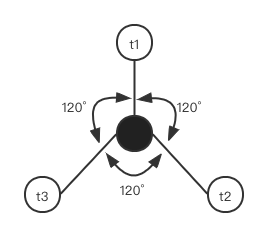
\includegraphics[scale=0.5]{img/pic2.png}
        \caption{斯坦纳树}
        \label{pic2}
    \end{minipage}
\end{figure}

\section{斯坦纳树的构造}

对于斯坦纳树构造的认识,科学家有着由简到繁的递进式推进过程。

意大利的托里切利最早解决了 $n=3$ 的斯坦纳树构造问题。
托里切利指出:若在 $ \triangle  ABC$ 的三条边上分别向外作一等边三角形,并对每一三角形作一外接圆,则此三圆交于一点 $P$ ,
即为所求之点。但这只适用于三点所构成的三角形内角均小于 $120^{\circ}$ 的情形。
1647年,意大利的卡瓦列里(F.B.Cavalieri)进一步证明了上述作图中,在 $P$ 点的三个交角 $\angle  APB$,$\angle BPC$ 和 $\angle CPA$ 均为 $120^{\circ}$ 。
1834年海嫩(F.Heinen)提出并解决了存在一内角 $\leq  120^{\circ}$的情形。此种情况为一退化情况,此时的点P应选在三角形最大内角的角顶。

对于 $n=4$ 的情况要比 $n=3$ 时复杂得多,对于三点来说,斯坦纳树的可能连接方式有4种,但是对于四点来说,可能的连接方式就达到了31\cite{2} 种。对此,1978 年波拉克(H.O.Pollak) 给出了一波拉克定理。

对于 $n=4$ 时,一般存在2株斯坦纳树,总长一般不相等,通过波拉克定理可不必求出两株树再进行比较,但对于 $n \geq 5$ 时,还没有发现这样的方法。并且已证明寻求 $SMT(X)$ 为一NP难题。目前所用的方法基本是枚举法。此时点集所组成的归类迅速增大。如当 $n=6$ 时, 其数为5625,而当 $n=8$ 时则达到2643795。因而目前这类问题主要有两种解决途径:一是 对 $X$ 的性质加些限制:二是寻求问题的近似解。

\section{算法实现}

\subsection{最小斯坦纳树}

\subsubsection*{题目描述}

\begin{quotation}
    给定一个包含 $n$ 个结点和 $m$条带权边的无向连通图 $G=(V,E)$ 。

    再给定包含 $k$ 个结点的点集 $S$,选出 $G$ 的子图 $G'=(V',E')$ ,使得:
    \begin{enumerate}
        \item $S \subseteq V'$ ;
        \item $G'$ 为连通图;
        \item $E'$ 中所有边的全值和最小。
    \end{enumerate}

    你只需要求出 $E'$ 中所有边的权值和。
\end{quotation}

\subsubsection*{样例}

$n=7,\ m=7,\ k=4$

红色点为 $S$ 中的元素,红色边为 $E'$ 的元素,此时 $E'$ 中所有边的权值和为 $2+2+3+4=11$ ,达到最小值。

\begin{figure}[htbp]
    \centering
    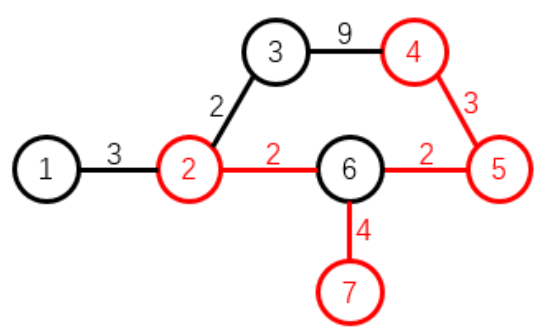
\includegraphics{img/pic3.png}
    \caption{最小斯坦纳树样例}
    \label{pic3}
\end{figure}

\subsubsection*{题解}

结合上面的知识可以知道直接连接 $k$ 个关键点生成的权值和不一定是最小的,或者这 $k$ 个关键点不会直接连接。
所以应当使用剩下的 $n-k$ 个关键点不会直接连接。

这里考虑使用状态压缩动态规划来求解。用 $f(i,S)$表示以 $i$ 为根的一棵树,包含集合 $S$ 中所有点点最小边权值和。

考虑状态转移:
\begin{itemize}
    \item 首先对连通的子集进行转移,$f(i,S) \leftarrow min(f(i,S),f(i,T)+f(i,S-T))$
    \item 在当前的子集连通状态下进行边点松弛操作,$f(i,S) \leftarrow min(f(i,S),f(j,S)+w(j,i))$。用 `tree[tot]` 来记录两个相连节点 $i,j$ 的相关信息。
\end{itemize}

\subsubsection*{Code}

\begin{lstlisting}
#include <bits/stdc++.h>

using namespace std;

const int maxn = 510;
const int INF = 0x3f3f3f3f;
typedef pair<int, int> P;
int n, m, k;

struct edge {
    int to, next, w;
} e[maxn << 1];

int head[maxn << 1], tree[maxn << 1], tot;
int dp[maxn][5000], vis[maxn];
int key[maxn];
priority_queue<P, vector<P>, greater<P> > q;

void add(int u, int v, int w) {
    e[++tot] = edge{v, head[u], w};
    head[u] = tot;
}

void dijkstra(int s) {  // 求解最短路
    memset(vis, 0, sizeof(vis));
    while (!q.empty()) {
    P item = q.top();
    q.pop();
    if (vis[item.second]) continue;
    vis[item.second] = 1;
    for (int i = head[item.second]; i; i = e[i].next) {
        if (dp[tree[i]][s] > dp[item.second][s] + e[i].w) {
        dp[tree[i]][s] = dp[item.second][s] + e[i].w;
        q.push(P(dp[tree[i]][s], tree[i]));
        }
    }
    }
}

int main() {
    memset(dp, INF, sizeof(dp));
    scanf("%d %d %d", &n, &m, &k);
    int u, v, w;
    for (int i = 1; i <= m; i++) {
    scanf("%d %d %d", &u, &v, &w);
    add(u, v, w);
    tree[tot] = v;
    add(v, u, w);
    tree[tot] = u;
    }
    for (int i = 1; i <= k; i++) {
    scanf("%d", &key[i]);
    dp[key[i]][1 << (i - 1)] = 0;
    }
    for (int s = 1; s < (1 << k); s++) {
    for (int i = 1; i <= n; i++) {
        for (int subs = s & (s - 1); subs;
            subs = s & (subs - 1))  // 状压 dp 可以看下题解里写的比较详细
        dp[i][s] = min(dp[i][s], dp[i][subs] + dp[i][s ^ subs]);
        if (dp[i][s] != INF) q.push(P(dp[i][s], i));
    }
    dijkstra(s);
    }
    printf("%d\n", dp[key[1]][(1 << k) - 1]);
    return 0;
}
\end{lstlisting}

\subsection{[WC2008]游览计划}

\subsubsection*{题目描述}

这道题是求点权和最小的斯坦纳树,用 $f(i,S)$ 表示以 $i$ 为根的一棵树,包含集合 $S$ 中所有点的最小点权值和。$a_i$ 表示点权。

考虑状态转移:
\begin{itemize}
    \item $f(i,S) \leftarrow min(f(i,S),f(i,T)+f(i,S-T)-a_i)$ 。由于此处合并时同一个点 $a_i$,会被加两次,所以减去。
    \item $f(i,S) \leftarrow min(f(i,S),f(j,S)+w(j,i))$ 。
\end{itemize}

可以发现状态转移与最小斯坦纳树的模板题是类似的,麻烦的是对答案的输出,在 $DP$ 的过程中还要记录路径。

\subsubsection*{Code}

\begin{lstlisting}
#include <bits/stdc++.h>

using namespace std;

#define mp make_pair
typedef pair<int, int> P;
typedef pair<P, int> PP;
const int INF = 0x3f3f3f3f;
const int dx[] = {0, 0, -1, 1};
const int dy[] = {1, -1, 0, 0};
int n, m, K, root;
int f[101][1111], a[101], ans[11][11];
bool inq[101];
PP pre[101][1111];
queue<P> q;

bool legal(P u) {
    if (u.first >= 0 && u.second >= 0 && u.first < n && u.second < m) {
    return true;
    }
    return false;
}

int num(P u) { return u.first * m + u.second; }

void spfa(int s) {
    memset(inq, 0, sizeof(inq));
    while (!q.empty()) {
    P u = q.front();
    q.pop();
    inq[num(u)] = 0;
    for (int d = 0; d < 4; d++) {
        P v = mp(u.first + dx[d], u.second + dy[d]);
        int du = num(u), dv = num(v);
        if (legal(v) && f[dv][s] > f[du][s] + a[dv]) {
        f[dv][s] = f[du][s] + a[dv];
        if (!inq[dv]) {
            inq[dv] = 1;
            q.push(v);
        }
        pre[dv][s] = mp(u, s);
        }
    }
    }
}

void dfs(P u, int s) {
    if (!pre[num(u)][s].second) return;
    ans[u.first][u.second] = 1;
    int nu = num(u);
    if (pre[nu][s].first == u)
    dfs(u, s ^ pre[nu][s].second);  //通过 dfs 来找到答案
    dfs(pre[nu][s].first, pre[nu][s].second);
}

int main() {
    memset(f, INF, sizeof(f));
    scanf("%d %d", &n, &m);
    int tot = 0;
    for (int i = 0; i < n; i++) {
    for (int j = 0; j < m; j++) {
        scanf("%d", &a[tot]);
        if (!a[tot]) {
        f[tot][1 << (K++)] = 0;
        root = tot;
        }
        tot++;
    }
    }
    for (int s = 1; s < (1 << K); s++) {
    for (int i = 0; i < n * m; i++) {
        for (int subs = s & (s - 1); subs; subs = s & (subs - 1)) {
        if (f[i][s] > f[i][subs] + f[i][s ^ subs] - a[i]) {
            f[i][s] = f[i][subs] + f[i][s ^ subs] - a[i];  // 状态转移
            pre[i][s] = mp(mp(i / m, i % m), subs);
        }
        }
        if (f[i][s] < INF) q.push(mp(i / m, i % m));
    }
    spfa(s);
    }
    printf("%d\n", f[root][(1 << K) - 1]);
    dfs(mp(root / m, root % m), (1 << K) - 1);
    for (int i = 0, tot = 0; i < n; i++) {
    for (int j = 0; j < m; j++) {
        if (!a[tot++])
        putchar('x');
        else
        putchar(ans[i][j] ? 'o' : '_');
    }
    if (i != n - 1) printf("\n");
    }
    return 0;
}
\end{lstlisting}

\subsection{Other}

还有相关的Online Judge习题:

\begin{itemize}
    \item {[JLOI 2015]} 管道连接
    \item {[APIO 2013]} 机器人
    \item {[HDU 4085]} Peach Blossom Spring
    \item {[ZOJ 3613]} Wormhole Transpor
\end{itemize}

\section{现实应用}

\subsection{无线传感器网络连通恢复}

目前,无线传感器的使用日渐广泛,正常情况下,无线传感器作为节点相互连接形成通信链路,组成网络正常运转。
而在一些意外情况下,节点失效,网络被分割为若干个无法通信的区域。
这时候,如果可以在实现恢复连通的情况下,尽可能少的布置中继节点是该问题着力解决的目标。而这个问题是一个NP难题,实际情形下多数使用启发式算法。

而斯坦纳树就可以很好的应用到其中。
已经有相关研究人员提出基于斯坦纳树的算法,试图去确定斯坦纳点,以四边形斯坦纳树,三角形斯坦纳树或者最小生成树去找到最少的中继节点的集合,完成对无线传感器网络的恢复。
此恢复方法对类似的网络的鲁棒性研究有着相似之处,有着重要的应用价值。

\subsection{北京冬奥会志愿者安排}

在思考斯坦纳树相关问题过后,联想到它可能在现实的应用场景。

假设在北京冬奥会有许多比赛场地和场馆,它们分布在各个地方,运动员在比赛场地和场馆之间移动时,最好有志愿者进行服务。
我们将这个现实问题抽象到一个二维平面上,地图是一个 $n*m$ 的长方形,地点是地图上一个个方块。
理想情况下希望,保证任两个地点之间,存在一条路径,这条路径上所进过的每一个方块都有志愿者。
当然志愿者的数量是有限的,所以我们希望志愿者的数量可以尽可能的少,请问如何安排志愿者?

很明显,这个问题可以套用最小斯坦纳树的模版,再结合现实问题的限制进行计算。

\section{结论}

结合斯坦纳树问题相关历史资料,文献以及Online Judge上与之相关的问题,对斯坦纳树的了解更加透彻。
对最小斯坦纳树的问题进行时实际的研究和解决,经历了一个从无知到了解到比较深刻的理解的过程。
这次综述深化并扩展了相关的知识体系结构,相信这对今后的学习与研究工作将会产生非常有益的影响。
而斯坦纳树问题会在现在的各项相关应用越来越多的应用并延伸,发挥着重要的作用。

%文献研究的结论,概括指出自己对该课题的研究意见,存在的不同意见和有待解决的问题等;

%%%%%%%%%%%%%%%%%%%%%%%%%%%%%%%%%%%%%%%%%%%%%%%%%%%%%%%
%%% 致谢
%%% 非必选
%%%%%%%%%%%%%%%%%%%%%%%%%%%%%%%%%%%%%%%%%%%%%%%%%%%%%%%
%\Acknowledgements{致谢.}

%%%%%%%%%%%%%%%%%%%%%%%%%%%%%%%%%%%%%%%%%%%%%%%%%%%%%%%
%%% 补充材料说明
%%% 非必选
%%%%%%%%%%%%%%%%%%%%%%%%%%%%%%%%%%%%%%%%%%%%%%%%%%%%%%%
%\Supplements{补充材料.}

%%%%%%%%%%%%%%%%%%%%%%%%%%%%%%%%%%%%%%%%%%%%%%%%%%%%%%%
%%% 参考文献, {}为引用的标签, 数字/字母均可
%%% 文中上标引用: \upcite{1,2}
%%% 文中正常引用: \cite{1,2}
%%%%%%%%%%%%%%%%%%%%%%%%%%%%%%%%%%%%%%%%%%%%%%%%%%%%%%%
\newpage

\begin{thebibliography}{99}

    \bibitem{1} Ljubi, Ivana . "Solving Steiner trees: Recent advances, challenges, and perspectives." Networks. 

    \bibitem{2} Dingzhu Du, Xiaodong Hu, Steiner Tree Problems in Computer Communication Networks, World Scientific, 2008.

    \bibitem{3} ShaoChenHeng, Enter-tainer. "斯坦纳树." (2021). 

    \bibitem{4} 越民义, 最小网络——斯坦纳树问题. 上海科学技术出版社, 2006.11.

    \bibitem{5} Courant,R., Robbins,H., 什么是数学. 科学出版社,1985.01.

\end{thebibliography}

%%%%%%%%%%%%%%%%%%%%%%%%%%%%%%%%%%%%%%%%%%%%%%%%%%%%%%%
%%% 附录章节, 自动从A编号, 以\section开始一节
%%% 非必选
%%%%%%%%%%%%%%%%%%%%%%%%%%%%%%%%%%%%%%%%%%%%%%%%%%%%%%%
%\begin{appendix}
%\section{附录}
%附录从这里开始.
%\begin{figure}[H]
%\centering
%%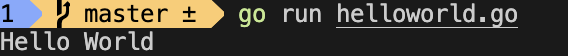
\includegraphics{fig1.eps}
%\cnenfigcaption{附录里的图}{Caption}
%\label{fig1}
%\end{figure}
%\end{appendix}

\end{document}
